%%%%%%%% MID-SEMESTER UPDATE (WRITTEN) : EN.553.602 %%%%%%%%%%%%%%%%%%%%%%%%
\documentclass{article}

\usepackage{microtype}
\usepackage{graphicx}
\usepackage{booktabs}
\usepackage{hyperref}

\newcommand{\theHalgorithm}{\arabic{algorithm}}
\usepackage[accepted]{icml2026}
\renewcommand{\ttdefault}{cmtt}
% TinyTeX here lacks Courier (pcr); Computer Modern typewriter instead
% No affiliation/venue footnote on page 1 (not required for the course); tell the style it was handled
\makeatletter\global\icml@noticeprintedtrue\makeatother

\usepackage{amsmath}
\usepackage{amssymb}
\usepackage{tabularx}
\usepackage{array}
\usepackage[capitalize,noabbrev]{cleveref}

% Evidence labels used throughout (same meaning as on the midterm slides)
\newcommand{\lab}[1]{{\footnotesize\textsf{\textbf{#1}}}}
\newcommand{\OBS}{\lab{OBSERVED}}
\newcommand{\DER}{\lab{DERIVED}}
\newcommand{\ASM}{\lab{ASSUMED}}
\newcommand{\DES}{\lab{DESIGNED}}
\newcommand{\SIM}{\lab{SIMULATED}}
\newcolumntype{L}{>{\raggedright\arraybackslash}X}
\newcolumntype{P}[1]{>{\raggedright\arraybackslash}p{#1}}
\renewcommand{\arraystretch}{1.12}

\icmltitlerunning{Optimizing the Night Ride: Mid-Semester Update}

\begin{document}

\twocolumn[
\icmltitle{Optimizing the Night Ride: Mid-Semester Update\\ When Should Blue Jay Night Ride Move a Waiting Request to Lyft?}

  \begin{icmlauthorlist}
    \icmlauthor{Irfan Setiadi}{}
    \icmlauthor{Miles Zhou}{}
    \icmlauthor{Youzhi Zhang}{}
    \icmlauthor{Vignesh Rajesh Babu}{}
  \end{icmlauthorlist}


\vskip 0.05in
\begin{center}\small
Team FourSight \quad$\cdot$\quad Department of Applied Mathematics and Statistics, Johns Hopkins University\\
EN.553.402\,/\,553.602 Research and Design in Mathematics: Data Mining \quad$\cdot$\quad Instructor: Prof.\ Anthony J.\ Kearsley \quad$\cdot$\quad Fall 2026
\end{center}
\vskip 0.2in
]


\begin{abstract}
Blue Jay Night Ride is Johns Hopkins' on-demand, shared evening van service. When the vans fall behind, a dispatcher can move a waiting request to a paid Lyft. Our proposal planned to replay real service nights from trip-level records and to compare dispatch algorithms head to head. The trip-level records never arrived; the only operational data are April 2026 aggregate dashboards. This report describes what we did instead. We turned the aggregates into a set of plausible synthetic evenings, labelling every input as observed, derived, assumed or designed. We built an event simulator and a van dispatcher: an exact mixed-integer linear program (MILP) over a restricted set of candidate routes, solved repeatedly within a rolling-horizon heuristic. We narrowed the research question to one controllable decision: with the van dispatcher held fixed, when should a waiting request move to Lyft? In a controlled two-van pilot (30 constructed nights, each replayed under six transfer rules), the two rules that read the van plan's predicted pickup reached about three quarters of requests within 15 minutes (a van or Lyft at the curb within 15 minutes of the request), against about half with vans only, while ordering roughly 9 to 10.5 Lyft rides per night. Most of that gain comes from moving requests to Lyft early; whether the prediction itself adds value at an equal Lyft budget is not yet tested. No rule was best on both service and Lyft use. These are verified simulation results under provisional assumptions, not a policy recommendation; the report closes with the robustness tests and the dispatcher benchmark planned for the final.
\end{abstract}

% =====================================================================
\section{Introduction}\label{sec:intro}

\textbf{The service.} Homewood-area Night Ride pools requests from students, faculty and staff into shared 14-seat vans in the evening. A rider books through the TransLoc app, a van is routed to the curb, and the rider is dropped at their destination. When demand outruns the vans, a dispatcher can transfer a waiting request to Lyft. The rider then waits for the Lyft instead, and Hopkins pays for an extra trip. Our study area is the Homewood service including the Peabody area; East Baltimore is excluded. Trip ends follow April's maps, which include a few places further south, such as the Inner Harbor.

\textbf{One request.} A request may carry several passengers. Waiting time runs from the request to the moment a vehicle reaches the curb (\emph{curb arrival}). A rider who gives up before then is a \emph{cancellation}. A rider absent after a 3-minute curb wait is a \emph{no-show}. A request moved to Lyft becomes a separate Lyft order, and the rider can still cancel or be absent.

\textbf{The question.} The April data show long tail waits and heavy Lyft use: the dashboards place the 90th-percentile wait for completed rides at about 17 to 21 minutes, and about 24.5\% of all riders travelled by Lyft \OBS{} (evidence labels such as \OBS{} say how we know a number; they are explained in \cref{sec:data}). Both point at the same lever, the decision to move a waiting request to Lyft. We therefore ask:

\begin{quote}\itshape
Holding one specified van dispatcher fixed, how do the timing and the information used by a Lyft transfer rule change rider service and Lyft use?
\end{quote}

\Cref{fig:system} shows the system. The van dispatcher and the transfer rule are policies; they see only what a real dispatcher could see. The simulator is the referee: it owns the clock and applies each rider's hidden traits (patience, presence at the curb, Lyft delay) only when the matching event happens.

\begin{figure*}[t]
\centering
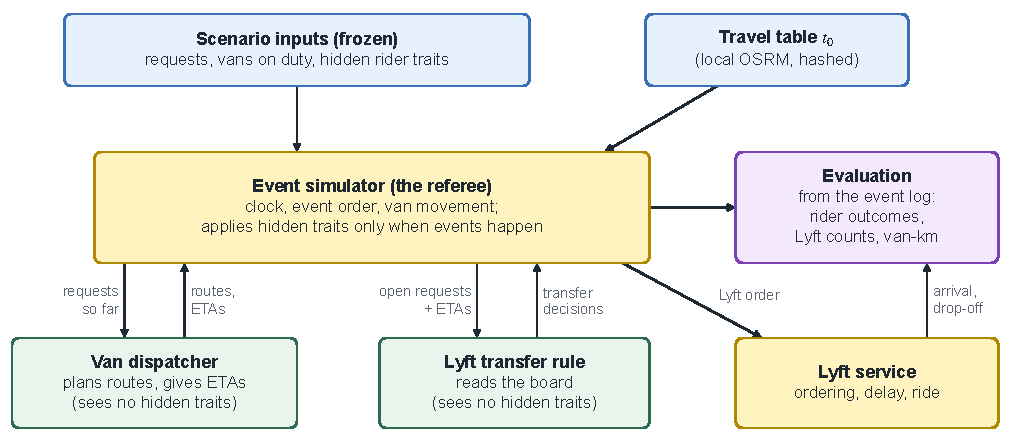
\includegraphics{figures/d_system.pdf}
\caption{The system in one picture. A frozen scenario and a travel-time table feed the event simulator, which acts as referee. $t_0$ is the fixed table of travel times between all 188 places (OSRM $\times$ 1.2); ``hashed'' means its content is fingerprinted so every run uses the same table. ETAs are the plan's predicted curb-arrival times, and ``reads the board'' means the rule sees the open requests and those predictions. The van dispatcher and the Lyft transfer rule (green) are the policies; they see only what a real dispatcher could see. The Lyft service is deliberately thin: the study needs \emph{when} a transferred rider is picked up, not how Lyft matches drivers.}\label{fig:system}
\end{figure*}

\textbf{Contributions to date.} (i) An evidence base of April aggregates, each number labelled by how we know it (\cref{sec:data}). (ii) A block-by-block recipe that turns those aggregates into synthetic evenings (\cref{sec:scenario}). (iii) A verified event simulator (checked against hand-computed cases to confirm the code implements the specified model; \cref{sec:design}) with a rolling-horizon mixed-integer linear programming (MILP) dispatcher, which re-plans at each decision moment using only what is known then (\cref{sec:sim}) and six transfer rules (\cref{sec:rules}). (iv) A 30-night, six-rule pilot with checked outputs (\cref{sec:design,sec:results}). We also report what did not work (\cref{sec:failed}), what could change the answer (\cref{sec:limits}) and the plan for the final (\cref{sec:plan}).

% =====================================================================
\section{Changes to the Original Plan}\label{sec:changes}

\textbf{What changed and why.} The proposal expected trip-level extracts so that real nights could be replayed, and it planned to compare greedy rules (each new request placed at its cheapest position on arrival and never reassigned), a rolling-horizon MILP and a hybrid on the same request stream, with Lyft overflow decided inside the optimizer. Three main things changed; \cref{tab:pivot} lists all five differences. The extracts never arrived, so every evening is synthetic. We narrowed the question to one controllable decision, holding a specified van dispatcher fixed, because the real dispatcher's internals are not known to us and a controlled comparison needs everything else held fixed. And Lyft became a separate, explicit transfer rule rather than a term in the van objective. Holding the dispatcher fixed is a scope choice: synthetic nights do not rule out comparing dispatch algorithms, and we plan to do so (\cref{sec:plan}).

\begin{table}[t]
\centering\small
\caption{From the September proposal to the current study.}\label{tab:pivot}
\begin{tabularx}{\columnwidth}{@{}P{2.25cm}L@{}}
\toprule
\textbf{Proposal} & \textbf{Now, and why}\\
\midrule
Replay real nights from trip-level records & Synthetic evenings built from April aggregates; the records did not arrive\\
Compare dispatch algorithms head to head & Compare Lyft transfer rules with one van dispatcher held fixed; a scope choice to isolate the rule\\
Lyft overflow minimized inside the MILP & A separate transfer rule; no money modelled, since Hopkins' cost per Lyft trip is unknown to us\\
Published targets as hard limits & Reporting thresholds, plus a ride-time guardrail\\
Claims about real nights & Claims about synthetic evenings consistent with April's totals, under stated assumptions\\
\bottomrule
\end{tabularx}
\end{table}

\textbf{Numbers we corrected.} Re-reading the dashboards showed that four numbers in our proposal were misread (\cref{tab:corrected}). The largest error was reading a 30-day total as an hourly rate.

\begin{table}[t]
\centering\small
\caption{Proposal numbers, corrected. Source: April 2026 dashboards (digitized aggregates).}\label{tab:corrected}
\begin{tabularx}{\columnwidth}{@{}P{2.3cm}L@{}}
\toprule
\textbf{Proposal said} & \textbf{Corrected}\\
\midrule
About 5,100 rides per hour at 6 pm & A 30-day total for the 6 pm hour (tooltip 5,098; digitized 5,089), about 170 completed rides in one evening's 6 pm hour\\
About 28 vans in service & 27.6 vehicles at 6 pm, the ``All services'' average; not a Homewood-only count\\
7 pm bar ``4,900'' & Our digitized value is 3,957, also a 30-day total\\
About 1 in 4 trips overflow to Lyft & 24.5\% of the 44,374 riders rode Lyft: a share of riders, not of trips or requests\\
\bottomrule
\end{tabularx}
\end{table}

\textbf{Response to the proposal feedback.} The professor's written comment on the proposal raised seven points. \Cref{tab:feedback} records where each now stands; its terms are defined in the sections it cites. The most important open one is the computational question of when the rolling-horizon MILP outperforms greedy assignment (greedy insertion, in our terms); our pivot set it aside, and we plan to answer it directly (\cref{sec:plan}).

\begin{table*}[t]
\centering\small
\caption{The professor's proposal feedback and where each point stands at the midterm. Terms used here are defined later: decision moments and candidate routes in \cref{sec:sim}, the cap $K$ and the postponement constant $M$ in \cref{sec:milp}, ``reached within 15 min'' in \cref{sec:reach}, greedy insertion in \cref{sec:plan} (item 6).}\label{tab:feedback}
\begin{tabularx}{\textwidth}{@{}P{4.4cm}P{1.9cm}L@{}}
\toprule
\textbf{Point raised} & \textbf{Status} & \textbf{What we did, or will do}\\
\midrule
Can optimization reduce waits and Lyft overflow? & Reframed; not yet tested & We study one controllable decision (the transfer rule) with the dispatcher fixed, so nothing here tests optimization itself. Rules that read the plan's prediction reached more requests in 15 min, largely by transferring early, but used more Lyft (\cref{sec:results}); the optimization question is item 6 of \cref{sec:plan}\\
When does the rolling-horizon MILP beat greedy; does the gap depend on fleet, demand, horizon? & Open & Planned benchmark: MILP vs greedy insertion on identical nights, across 4 to 7 vans, four demand patterns and re-planning intervals of 60 / 120 / 300 s (\cref{sec:plan}). Our ``horizon'' is all known work with no look-ahead, so the levers are re-planning interval and candidate cap\\
Does the dial-a-ride aspect make optimization valuable? & Plausible, untested & April's ride-time tail exceeds the longest direct drive, consistent with shared-ride detours, so routing choices plausibly matter. Only the benchmark can show it\\
Lexicographic or weighted objective? Risk of Lyft-first behaviour & Addressed & A weighted sum in passenger-minutes with a convex waiting penalty; Lyft is not in the van objective at all (\cref{sec:milp}). Service and Lyft use are reported as two objectives (\cref{sec:tradeoff}). Apart from a guardrail penalty $\Psi$ for excess that no route can avoid, one large ranking constant remains (the postponement constant $M$): it makes the solver postpone as few requests as its candidates allow before trading minutes\\
Make the Dial-a-Ride Problem clear & Addressed & Stated in \cref{sec:sim}: a dynamic, door-to-door dial-a-ride problem with shared vans, each pickup matched to its drop-off, capacity and ride-time limits\\
Clarify the time windows & Addressed & No hard pickup window; waiting is soft and priced; ride time has a guardrail; published targets are reporting thresholds (\cref{sec:milp})\\
Be careful with ``exact'' & Addressed & We say: an exact MILP over a restricted candidate set, solved repeatedly within a rolling-horizon heuristic, optimal over its candidates at each decision moment, subject to solver status\\
\bottomrule
\end{tabularx}
\end{table*}

% =====================================================================
\section{Data Acquisition and Preprocessing}\label{sec:data}

\textbf{What we have.} Johns Hopkins University (JHU) Transportation shared the April 2026 TransLoc operations dashboards for the Homewood Night Ride. They are restricted, so this report quotes only aggregate numbers. They contain: requests by final status, completed rides by hour (30-day totals), average vehicles on duty by hour, pickup and drop-off density maps with printed counts, and wait and ride-time percentiles. They never show one rider's request, wait and outcome together. We know \emph{how many} requests ended in each status, \emph{where} pickups and drop-offs accumulated, and \emph{how} activity varied by hour; we cannot reconstruct any single journey.

\textbf{Preprocessing.} We digitized every chart into tables. Two readers independently counted the map bubbles; they agreed on 214 of 215. The city maps sum to 24,056 origins and 24,057 destinations: origins and destinations agree to within one, and fall 39 and 38 short of the 24,095 completed rides. We carried these residuals rather than forcing them. The maps became 188 georeferenced places in 16 zones. Road travel times between all places come from a locally hosted Open Source Routing Machine (OSRM) server [9] (Maryland road network), multiplied by 1.2 for van and Lyft time \ASM. Every number then received one of four labels, used on every slide and throughout this report:
\begin{itemize}\setlength\itemsep{1pt}
\item \OBS: read directly from the dashboards;
\item \DER: computed from observed numbers;
\item \ASM: our modelling choice, to be tested;
\item \DES: an experiment setting we chose.
\end{itemize}
Outputs of the simulator are labelled \SIM. \Cref{tab:april} lists the April numbers the study relies on.

\begin{table}[t]
\centering\small
\caption{April 2026 aggregates used in this report. All are \OBS{} except the last block, which is \DER{} under stated assumptions.}\label{tab:april}
\begin{tabularx}{\columnwidth}{@{}Lr@{}}
\toprule
\textbf{Quantity} & \textbf{Value}\\
\midrule
Recorded requests (month) & 50,297\\
Completed & 24,095\\
``Canceled'' & 23,843 (47\%)\\
``No Show'' & 2,359 (4.7\%)\\
Completed rides, 6 pm hour (30 days; tooltip) & 5,098\\
Vehicles at 6 pm, ``All services'' & 27.6\\
Riders, van and Lyft & 44,374\\
Lyft share of riders & 24.5\%\\
Completed-ride wait, 90th percentile (range of readings) & $\sim$17--21 min\\
Ride time, 90th percentile & $\sim$24 min\\
\midrule
Van passengers per completed request & 1.386\\
Requests per completed ride & 2.087\\
Requests per vehicle-hour, 6/7/8 pm & 12.85 / 10.10 / 10.71\\
\bottomrule
\end{tabularx}
\end{table}

\textbf{What the data already say.} Three findings from this evidence shaped the design. Demand outruns service: about 47\% of requests end ``Canceled''. The ride-time tail is consistent with detours for shared riders: the 90th-percentile ride (23.9 min) is longer than the longest direct drive in the area (13.6 min). And Lyft use tracks cancellations closely across days (correlation 0.88), which is consistent with Lyft hand-offs being recorded as ``Canceled''.

% =====================================================================
\section{Building Synthetic Evenings}\label{sec:scenario}

Because many different nights produce the same totals, we do not reconstruct ``the'' April night. We build plausible evenings, one block at a time, each block stating its evidence, its assumption and its limitation. A \emph{scenario} contains inputs only; cancellations, no-shows and transfers are produced during the run, never written in. Each ingredient has its own seeded random stream, so every rule faces identical riders with identical hidden traits (common random numbers).

\subsection{How busy an evening should be}\label{sec:volume}
We copy April's \emph{load per vehicle}, hour by hour, rather than April's raw volume (\cref{fig:workload}). For the 6 pm hour: the dashboard tooltip gives 5,098 completed rides over 30 days (our digitized bar reads 5,089), about 170 per evening; each completed ride corresponds to 2.09 requests on average, so about 355 requests arrived in that hour; spread over 27.6 vehicles, that is 12.85 requests per vehicle-hour (computed without intermediate rounding from the tooltip value; the digitized value gives 12.83, and the hourly counts below are unchanged). This assumes the monthly request-to-completion ratio holds within the hour and that the ``All services'' vehicle count stands in for Homewood vans \ASM. It is an estimated workload, not observed arrivals. For a planned evening of five vans, multiplying each hour's load by five and rounding by the largest-remainder rule gives 64 / 50 / 54 = 168 requests from 18:00 to 21:00 (\cref{fig:volume}). Because the Homewood share of vehicles and the rate of repeat requests are unknown, a plausible range is about 150 to 260 requests. This five-van evening is designed but has not been run yet.

\begin{figure*}[t]
\centering
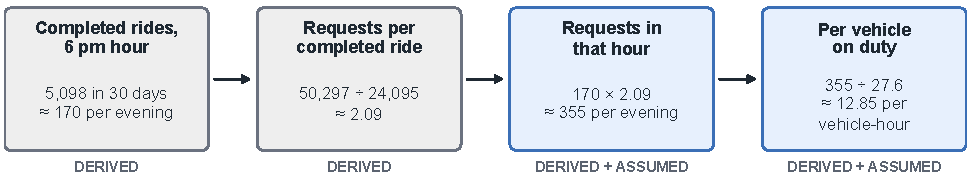
\includegraphics{figures/r1_workload.pdf}
\caption{From April totals to a workload per vehicle, 6 pm hour. Intermediate values are rounded for display. Grey boxes use only observed totals; blue boxes add the assumptions that the monthly request-to-completion ratio holds within the hour and that the ``All services'' vehicle count applies. The result is an estimated workload, not observed arrivals.}\label{fig:workload}
\end{figure*}

\begin{figure*}[t]
\centering
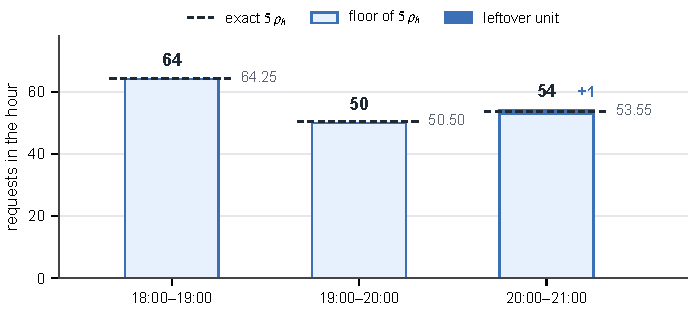
\includegraphics{figures/c_volume.pdf}
\caption{Hourly request counts for the planned five-van evening. Dashed lines are the exact values $5\rho_h$ (five vans times April's load per vehicle-hour); bars are the whole numbers used. Largest-remainder rounding gives the single leftover unit to 20:00--21:00, whose fraction (0.55) is largest: 64 / 50 / 54 = 168 \DER.}\label{fig:volume}
\end{figure*}

\subsection{The pilot: a smaller, deliberately demanding hour}\label{sec:pilot}
The results in this report come from a smaller pilot, built to test the whole pipeline before the five-van evening: \textbf{2 vans, 14 seats each, 28 requests between 18:00 and 19:00, repeated across 30 constructed nights} \DES. Of the 28 requests, 11 are placed in a 10-minute burst from 18:20 to 18:30 and 17 are spread over the hour; background requests can also fall in the burst window, so 11 to 17 requests (mean 13.7) arrive there on a given night (\cref{fig:arrivals}). Nights carry 34 to 51 passengers. The load, 14 requests per van-hour, is close to the 12.85 estimated for 6 pm, but the burst deliberately concentrates demand and two vans are a small fleet. This is a controlled pilot, not a reconstruction of a typical April night.

\begin{figure}[t]
\centering
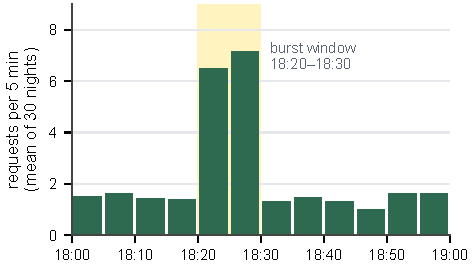
\includegraphics{figures/r2_arrivals.pdf}
\caption{Request arrivals in the pilot hour: requests per 5-minute bin, averaged over the 30 constructed nights (840 requests in all) \DES. The shaded burst window holds 13.7 requests per night on average.}\label{fig:arrivals}
\end{figure}

\subsection{Where trips start and end}\label{sec:pairing}
The maps give how many trips start and end at each place, not which start goes with which end (the origin-destination matching). Two different sets of trips can produce exactly the same totals (\cref{tab:toy}). The matching is therefore \emph{not identified} by the data; we must assume it. We assumed nearby journeys are more likely: an origin-destination pair's weight falls by a factor of about 0.9 for each extra minute of driving (rate 0.1 per minute) \ASM. We then normalized both sets of location totals to shares and rescaled rows and columns in turn (iterative proportional fitting [13]) until both were matched, to within $10^{-10}$. \Cref{fig:map} shows one constructed hour.

\begin{table}[t]
\centering\small
\caption{Two trip tables with identical place totals (illustration, not project data). The totals are all the maps show; both versions match them.}\label{tab:toy}
\begin{tabular}{@{}lccc@{\hspace{1.4em}}lccc@{}}
\toprule
\multicolumn{4}{c}{Version 1} & \multicolumn{4}{c}{Version 2}\\
\cmidrule(r{1.2em}){1-4}\cmidrule{5-8}
 & X & Y & total & & X & Y & total\\
\midrule
A & 2 & 0 & 2 & A & 1 & 1 & 2\\
B & 0 & 2 & 2 & B & 1 & 1 & 2\\
total & 2 & 2 & 4 & total & 2 & 2 & 4\\
\bottomrule
\end{tabular}
\end{table}

\begin{figure}[t]
\centering
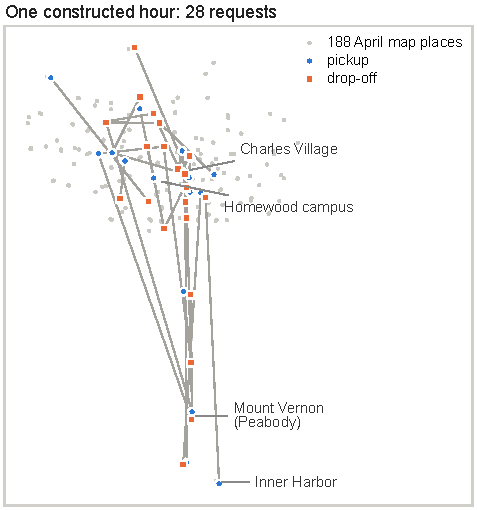
\includegraphics{figures/c_map.pdf}
\caption{One constructed pilot hour (night r00, the first of the 30): 28 requests drawn as straight pickup-to-drop-off links over the 188 April map places \DER{} + \ASM. Most trips stay near Homewood and Charles Village; a few reach Mount Vernon (Peabody) and the Inner Harbor. Geometry is schematic, without a basemap.}\label{fig:map}
\end{figure}

\subsection{Group sizes}\label{sec:groups}
April identifies an \emph{average}, 1.386 van passengers per completed van request \DER, not the distribution of group sizes. We chose shares of 73\% / 18\% / 5.5\% / 2.5\% / 1\% for parties of one to five (mean 1.405) \ASM. It covers all requests, while 1.386 covers completed van requests only; we chose a mean close to the observed one, and the small difference is our choice, not evidence. Many shapes share the same mean; the share of groups of three or more could plausibly range from 8\% to 12\% or more. Groups matter because they use seats and because waiting is counted per passenger. A party of five transferred to Lyft rides together in one Lyft XL (a larger Lyft vehicle) (a team decision, not verified Hopkins policy).

\subsection{Cancellations and patience}\label{sec:patience}
23,843 of 50,297 requests (47\%) ended ``Canceled'' \OBS. The label alone does not say whether the rider gave up or a dispatcher moved the request to Lyft. We assume Lyft transfers are also recorded as ``Canceled'', and we carry the share that is riders giving up as a range, 50--75\% \ASM. In the simulator each rider has a private patience deadline the dispatcher cannot see; if no vehicle reaches the curb by then, the rider cancels. The deadline keeps running after a transfer. The placeholder distribution is Weibull with shape 1.5 (impatience rising with time) and median 18 minutes (\cref{fig:assumed}, middle) \ASM. It lets the simulator represent abandonment; it is not a behavioural distribution measured from April, and many patience distributions could produce the same cancellation share. One check is already possible. April implies that riders giving up account for 0.474 $\times$ (50--75\%) = 23.7--35.6\% of requests. In our pilot under vans only, where every cancellation is a rider giving up, the share is 10.8 of 28 = 38.6\%, above that range. Part of the gap is the designed burst with two vans; part may be the placeholder itself. The first step of our plan tests other patience shapes and checks which bring this share inside April's range (\cref{sec:plan}).

\begin{figure*}[t]
\centering
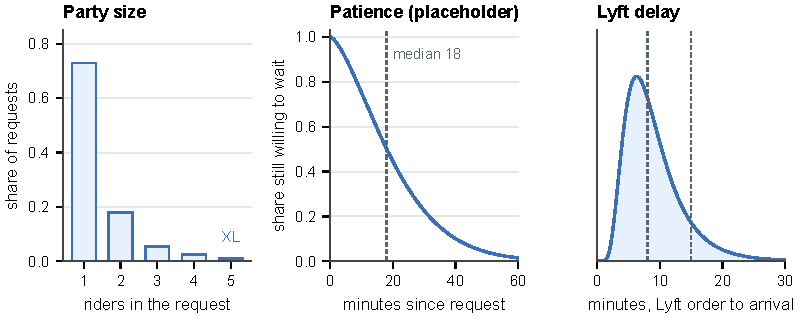
\includegraphics{figures/c_assumed.pdf}
\caption{Three assumed input distributions \ASM. Left: party-size shares per request. Middle: placeholder patience, shown as the share of riders still willing to wait after a given time. Right: Lyft delay from the Lyft order to its arrival at the curb (lognormal); dashed lines mark its median (8 min) and 90th percentile (about 15 min). None is a measured Hopkins distribution.}\label{fig:assumed}
\end{figure*}

\subsection{No-shows: the right denominator}\label{sec:noshow}
April's ``No Show'' share is 4.7\% of \emph{all} requests \OBS. But a no-show can only happen when a vehicle arrives, and the simulator needs a probability at that moment. Dividing the 2,359 no-shows by van arrivals (24,095 completed + 2,359 no-shows = 26,454) gives 8.9\% per arrival (\cref{fig:noshow}) \DER. The arithmetic is exact; the uncertainty lies in how statuses were recorded. The 8.9\% holds only if ``No Show'' was recorded after a real van arrival, ``Completed'' counts van trips, and Lyft hand-offs sit in ``Canceled''. The simulator gives each rider one hidden presence draw, used whichever vehicle arrives.

\begin{figure*}[t]
\centering
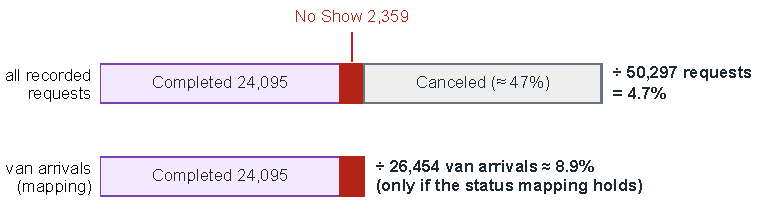
\includegraphics{figures/c_noshow.pdf}
\caption{Two denominators for the same 2,359 no-shows. Top: April's share of all recorded requests (4.7\%) \OBS. Bottom: the rate per van arrival (8.9\%), which holds only under the stated status mapping \DER. Applying 4.7\% at the curb would use the wrong denominator.}\label{fig:noshow}
\end{figure*}

\subsection{The blueprint}\label{sec:blueprint}
\Cref{tab:blueprint} gathers every input with its status. Inputs are fixed before a run; outcomes are not. Cancellations, no-shows and transfers happen during the run, from the hidden draws meeting the rule and the vans.

\begin{table}[!ht]
\centering\small
\caption{The scenario blueprint: every input and how we know it. ``Pilot'' marks where the pilot differs from, or adds to, the planned five-van evening; all other settings apply to both.}\label{tab:blueprint}
\begin{tabularx}{\columnwidth}{@{}P{2.0cm}P{2.0cm}L@{}}
\toprule
\textbf{Input} & \textbf{Status} & \textbf{Value}\\
\midrule
Requests per hour & \DER{} + \ASM & 64/50/54 for 5 vans; pilot 28 in one hour\\
Arrival times & \DER{} + \ASM & Uniform in the hour; pilot burst 18:20--18:30 \DES\\
Locations & \DER{} + \ASM & 188 April places\\
Trip matching & \ASM{} + \DER & Distance prior, balanced to map totals\\
Party sizes & \ASM & Shares chosen, mean 1.405 (close to the \DER{} 1.386)\\
Vans, seats & \DES & 5 planned (pilot 2), 14 seats\\
Travel times & \DER{} + \ASM & OSRM $\times$ 1.2\\
Patience & \ASM & Weibull 1.5, median 18 min\\
Presence & \DER{} + \ASM & 8.9\% absent per arrival\\
Lyft delay & \ASM & Lognormal, median 8 min\\
Ordering lag & \ASM & 2 min (pilot)\\
Rider accepts Lyft offer & \DES & Always (pilot)\\
Van dispatcher & \DES & Fixed (\cref{sec:sim})\\
Transfer rule & \DES & Varied: six rules (\cref{sec:rules})\\
\bottomrule
\end{tabularx}
\end{table}

% =====================================================================
\section{The Simulator and the Van Dispatcher}\label{sec:sim}

\textbf{The problem class.} The van side is a \emph{dynamic, door-to-door Dial-a-Ride Problem} [1--3, 5]: shared vans serve requests that arrive over time, each request is a pickup matched with a drop-off on the same van, pickup precedes drop-off, seats are limited, ride times are limited, and future requests are unknown.

\textbf{Three components with different jobs} (\cref{fig:arch}). The \emph{simulator} advances time and reveals events. The \emph{van optimizer} chooses among feasible candidate plans. The \emph{transfer rule} decides whether an eligible request (one still waiting for a van, not committed to one, and never having declined Lyft; \cref{sec:rules}) moves to Lyft.

\begin{figure*}[t]
\centering
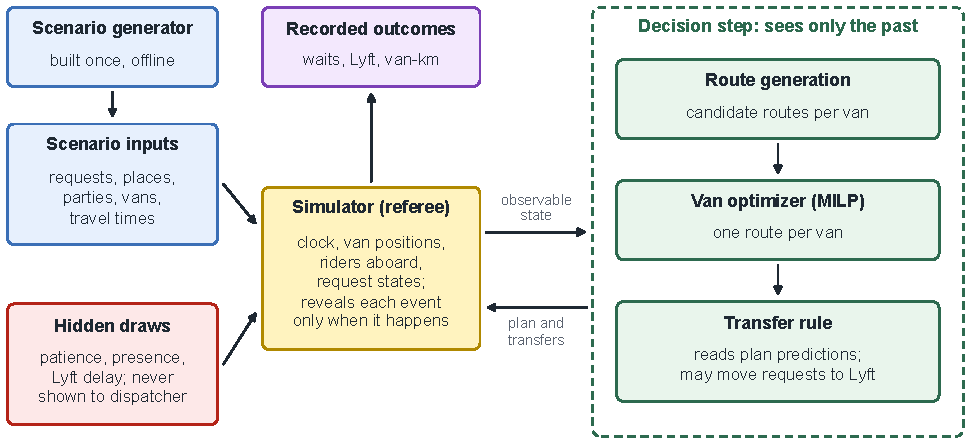
\includegraphics{figures/r5_architecture.pdf}
\caption{Simulator architecture. The generator builds scenario inputs and hidden draws once, offline. The simulator reveals a request only when it arrives and applies a hidden draw only when its event happens. At each decision step the dispatcher (route generation, then the MILP) and the transfer rule see only the observable state; vans then drive and commit to their next stop.}\label{fig:arch}
\end{figure*}

\textbf{The decision cycle.} The dispatcher sees requests that have arrived; it does not see future requests. A decision moment is triggered every 2 minutes and at each new request, each cancellation or no-show of a request waiting for a van, and each van coming on duty. At each moment: (1) new events are applied and the state observed; (2) a small set of feasible candidate routes (defined in \cref{sec:milp}) is generated for each van; (3) the MILP selects one route per van; (4) the transfer rule evaluates each request still waiting for a van; (5) accepted transfers leave van planning and the Lyft is ordered after a 2-minute lag; (6) the vans are re-planned once, only if a transfer happened; (7) vans depart, and a van commits to its next stop when it departs toward it. Only each van's next move is executed; the rest of the plan may change at the next moment. This is what we mean by \emph{rolling horizon}: the plan is re-optimized at every decision moment over all known requests, with no forecast of future requests, and only its first move is carried out. This re-planning design follows TransLoc's published 2016 description of its engine [10]; it is not verified current Hopkins practice. \Cref{fig:lifecycle} follows one request through these states, and Appendix~\ref{app:order} gives the order of events within one second.

\begin{figure*}[t]
\centering
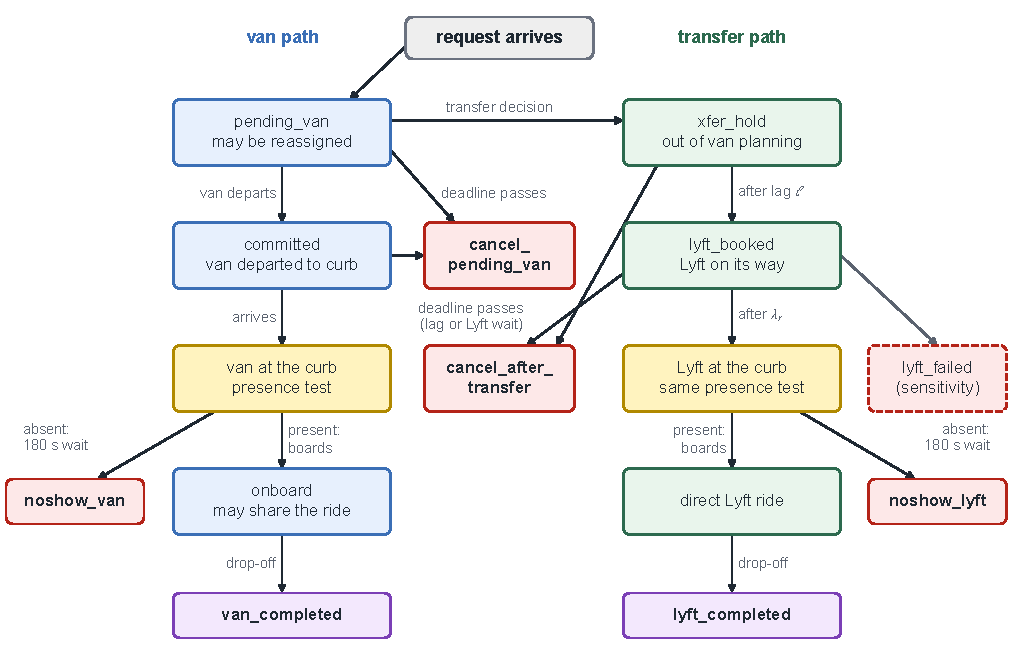
\includegraphics{figures/d_lifecycle.pdf}
\caption{The life of one request. Left: the van path. Right: the transfer path. Red boxes are terminal outcomes; the dashed box (\texttt{lyft\_failed}) is used only in a sensitivity case where a Lyft order can fail. $\ell$ is the ordering lag (2 minutes in the pilot) and $\lambda_r$ the rider's hidden Lyft delay; \texttt{lyft\_booked} means the Lyft has been ordered. ``Deadline passes'' is the hidden patience deadline. A rider can cancel while still waiting for a van and while a van is driving to the curb. During the 3-minute wait for an absent rider, the dispatcher plans as if the rider might still board; the simulator never boards an absent rider.}\label{fig:lifecycle}
\end{figure*}

\begin{figure*}[t]
\centering
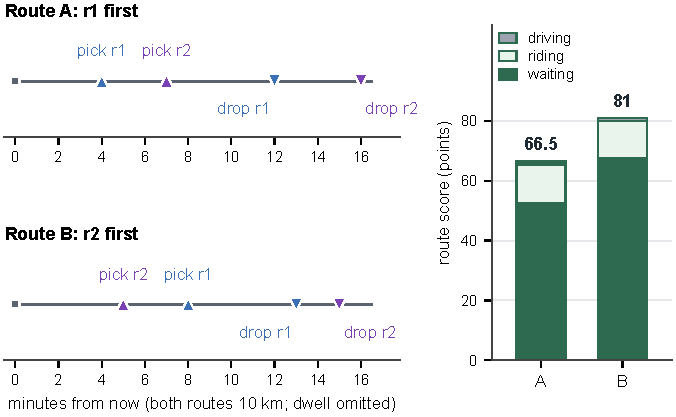
\includegraphics{figures/c_example.pdf}
\caption{Worked example (illustrative, computed by hand): two candidate routes for one van. Triangles pointing up are pickups, down are drop-offs; r1 is rider 1 and r2 the party of two in the text. Right: each route's score split into waiting, riding and driving points. Arithmetic in \cref{tab:example}.}\label{fig:example}
\end{figure*}


\subsection{The route-selection MILP}\label{sec:milp}
At each decision moment, for each van $v$ we build candidate routes $k$: every subset $S_{vk}$ of at most $K=3$ waiting requests, each placed in its best stop order (found by exact search over all the van's stops), plus the route containing only work already committed. Capacity, pickup before drop-off, commitments and the ride guardrail are enforced while routes are built. With $y_{vk}=1$ if van $v$ takes route $k$ and $u_r=1$ if request $r$ is postponed to a later decision moment:
\begin{equation}
\begin{aligned}
\min\ & \textstyle\sum_{v}\sum_{k} c_{vk}\, y_{vk} + \sum_{r} \pi_r\, u_r\\
\text{s.t. } & \textstyle\sum_{k} y_{vk} = 1 \qquad \forall v,\\
& \textstyle\sum_{v,k:\, r \in S_{vk}} y_{vk} + u_r = 1 \qquad \forall r,\\
& y_{vk},\ u_r \in \{0,1\}.
\end{aligned}\label{eq:milp}
\end{equation}
Here $r$ ranges over the waiting requests (not yet committed to a van), $c_{vk}$ is the route cost and $\pi_r$ the postponement price, both defined below. The first constraint gives each van exactly one route; the second serves each waiting request once or postpones it. This is the route-selection pattern of Alonso-Mora et al.\ [4], with ``drop the request'' replaced by ``postpone it at price $\pi_r$''. We solve it with the open-source HiGHS solver [8].

\textbf{Route cost, in points.} One point is one passenger-minute of waiting at the base slope. A route's cost combines four terms:
\begin{equation}
\begin{aligned}
c_{vk} ={}& \textstyle\sum_{r} q_r\, \varphi(W_r) + 0.5 \sum_{r} q_r H_r\\
&+ 0.1\,\text{km}_k + \Psi \textstyle\sum_r q_r (H_r - G_r)^{+},
\end{aligned}
\end{equation}
where the sums run over the requests served by route $k$ (new and committed), $q_r$ is party size, $W_r$ and $H_r$ are the total wait from the request and the ride time that route $k$ would give $r$, $\text{km}_k$ is the route's driving distance, $(x)^+ = \max(x,0)$, $G_r$ is the ride guardrail (below), and $\Psi = 1000$ points per passenger-minute a very large penalty for guardrail excess that no candidate can avoid. The weights are exchange rates: a riding minute is worth half a waiting minute at the base slope, and a kilometre is a small tie-breaker \ASM.

\textbf{Waiting is convex} (\cref{fig:phi}). $\varphi$ costs 1 point per minute for the first 5 minutes, then 2.5, 5, 10 and 20 points per minute after 5, 10, 15 and 20 minutes, so each extra minute costs more the longer the rider has already waited. Only part of this shape is evidenced: TransLoc's 2016 example [10] prefers cutting one minute from a 10-minute wait over two minutes from a 5-minute wait, which a straight line fails and our slopes pass ($2.5 > 2$). The rest is our choice \ASM. Because $\varphi$ is evaluated while route costs are computed, the optimization stays linear whatever its shape.

\begin{figure}[t]
\centering
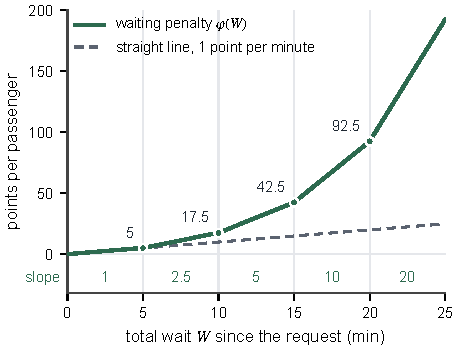
\includegraphics{figures/c_phi.pdf}
\caption{The convex waiting penalty $\varphi(W)$ per passenger. The slope rises at 5, 10, 15 and 20 minutes; the dashed line is a constant 1 point per minute for comparison \ASM.}\label{fig:phi}
\end{figure}

\textbf{Weighted, not lexicographic.} The proposal's ordering ``first cut Lyft overflow, then rider wait, then extra ride time, then distance'' read as lexicographic. We replaced it with the weighted sum above, for two reasons. A strict priority on waiting can buy a tiny wait saving with an unbounded on-board detour, the kind of long-ride tail that April's 24-minute ride percentile may partly reflect. And Lyft no longer appears in the van objective at all; it is decided by a separate, explicit rule (\cref{sec:rules}), so a small reduction in Lyft use cannot silently purchase a large increase in waiting. The service-versus-Lyft trade-off is instead reported openly (\cref{sec:tradeoff}).

\textbf{Time windows.} There is no hard pickup window. Waiting is soft and priced from the request time by $\varphi$; a transfer never resets the clock. Ride time has a guardrail $G_r = \max(25\text{ min},\ 2T_r + 5\text{ min})$, where $T_r$ is the direct drive: no candidate route may create or worsen a guardrail excess, and any excess already locked into committed work is charged $\Psi$ and logged. The published targets (15-minute pickup, 20-minute ride and 20-minute arrival at the destination during busy times on the pages captured around April; 20 / 25 / 25 minutes for the same three on the live page read in October [11]) are reporting thresholds, not constraints, since hard limits would be stricter than the service delivers.

\textbf{Postponement price.} $\pi_r = b_r + M$. Under the adopted rule (\cref{sec:pending}), $b_r = q_r\,\varphi(W_r^{\mathrm{early}})$, where $W_r^{\mathrm{early}}$ is the wait if $r$ were picked up at the earliest time any on-duty van could physically reach it (and no earlier than the next decision moment). $M$ is a large constant computed at each moment (Appendix~\ref{app:milp}). It guarantees that every proven-optimal plan postpones the fewest requests its candidates allow; only then does the solver trade minutes. This is the one near-lexicographic element left in the model, and it ranks van service, not Lyft.

\textbf{Worked example} (\cref{fig:example,tab:example}). One van, two waiting requests: rider 1 has waited 8 minutes; a party of two has waited 1 minute. Serving rider 1 first scores 66.5 points; serving the pair first scores 81.0, because rider 1's wait would cross 15 minutes, where each minute costs 10 points. The convex penalty protects the long waiter even though the other request carries two passengers.



\begin{table}[t]
\centering\small
\caption{Worked example arithmetic (minutes; both routes 10 km; dwell, the time stopped at the curb for boarding, omitted). $\varphi(12)=27.5$, $\varphi(8)=12.5$, $\varphi(16)=52.5$, $\varphi(6)=7.5$.}\label{tab:example}
\begin{tabularx}{\columnwidth}{@{}P{1.35cm}LL@{}}
\toprule
 & \textbf{A: rider 1 first} & \textbf{B: pair first}\\
\midrule
Waits & 12; 8 & 16; 6\\
Rides & 8; 9 & 5; 10\\
Waiting & $27.5 + 2(12.5) = 52.5$ & $52.5 + 2(7.5) = 67.5$\\
Riding & $0.5(8 + 18) = 13.0$ & $0.5(5 + 20) = 12.5$\\
Driving & 1.0 & 1.0\\
\midrule
\textbf{Total} & \textbf{66.5} & \textbf{81.0}\\
\bottomrule
\end{tabularx}
\end{table}

\textbf{What ``optimal'' means here.} We describe the dispatcher as an exact MILP over a restricted candidate set, solved repeatedly within a rolling-horizon heuristic. At each decision moment HiGHS proves optimality over the candidates generated then. The plan is not optimal over all routes (routes outside the candidate set are never considered), and not optimal for the evening (each moment is solved with what is known then). The cap $K=3$ is a tractability choice: exact ordering with four new pickups took minutes per decision moment in Python.



\subsection{A flaw we found and fixed: the postponement price}\label{sec:pending}
Our first formulation priced postponement as if the request would be served at the next 2-minute decision moment. That is earlier than any van could physically arrive, while a served request is charged its real, later pickup. Postponing could therefore look cheaper than serving. On a designed evening at 18:15, a party of five that had already waited 15 minutes was charged 262.5 points for postponement, against 435.8 points for the earliest physically possible pickup (18:19:28). A long-waiting party could be left waiting.

We compared three formulations on that whole evening, vans only (\cref{tab:pending}). The third, route-based price charges the request as if served after the van finishes its current route, which needs extra variables. We provisionally adopted the second: price postponement at the earliest time any on-duty van could physically reach the request. It changes cost coefficients only, adding no variables. In this one designed case (one run per formulation, $n = 1$) it reduced the worst wait from 44.4 to 35.6 minutes, while the median rose from 17.1 to 18.6; it did not reduce average waiting, and the longest waits fell while some younger requests waited longer. It is still optimistic, because it ignores the competing work of the van that could arrive first, and none of the three guarantees a feasible schedule for all waiting riders.

\begin{table}[t]
\centering\small
\caption{Three postponement prices on one designed evening, vans only, one run each \DES{} \SIM. Waits over requests picked up.}\label{tab:pending}
\begin{tabularx}{\columnwidth}{@{}Lccc@{}}
\toprule
 & \textbf{First} & \textbf{Adopted} & \textbf{Route-based}\\
\midrule
Priced as served at & next re-plan & earliest van & after a route\\
Wait median (min) & 17.1 & 18.6 & 21.1\\
Wait 90th percentile (min) & 31.0 & 31.2 & 34.3\\
Worst wait (min) & 44.4 & 35.6 & 38.6\\
Mean wait (min) & 18.8 & 18.8 & 21.8\\
Extra variables & 0 & 0 & up to 9,828\\
\bottomrule
\end{tabularx}
\end{table}

% =====================================================================
\section{The Lyft Transfer Rules}\label{sec:rules}

\begin{table*}[t]
\centering\small
\caption{The six transfer rules. ``Predicted total wait'' is the van plan's predicted pickup clock time minus the request clock time; a request with no feasible van counts as infinitely late, so the rule fires. Codes are used in figures; the number in a code is the threshold in minutes (for R3, the margin by which the van must be later than Lyft). A request is unassigned when no selected van route contains it (it was postponed, \cref{sec:milp}). Expected Lyft pickup = decision time + 2-minute ordering lag + 8-minute median Lyft delay.}\label{tab:rules}
\begin{tabularx}{\textwidth}{@{}P{4.6cm}P{1.3cm}P{3.6cm}L@{}}
\toprule
\textbf{Rule} & \textbf{Code} & \textbf{Information used} & \textbf{Transfers when}\\
\midrule
Vans only & R0 & none & never\\
Wait ten minutes & R1(10) & time already waited & now $-$ request time $\ge$ 10 min\\
Wait fifteen minutes & R1(15) & time already waited & now $-$ request time $\ge$ 15 min\\
Unassigned for ten minutes & R1u(10) & time outside every van plan & continuously unassigned $\ge$ 10 min (resets when assigned)\\
Predicted total wait exceeds fifteen minutes & R2(15) & van plan's prediction & predicted total wait $>$ 15 min\\
Lyft arrives sooner & R3(2) & prediction + typical Lyft delay & predicted van pickup later than expected Lyft pickup by $>$ 2 min\\
\bottomrule
\end{tabularx}
\end{table*}

We change the transfer decision, not the van dispatcher. A request is eligible while it is still waiting for a van, not committed to one, and has never declined a Lyft offer; rules are evaluated once per decision moment, after the dispatcher's solve. \Cref{tab:rules} defines the six rules. The thresholds were specified before any run and not changed after seeing results. The rules fall into three groups: the \emph{waiting-time rules} look only at time already waited; ``Unassigned for ten minutes'' looks at how long a request has been left outside every van plan; the \emph{predictive rules} read the van plan's predicted pickup. For a postponed request the predicted pickup is a tentative estimate, not a planned stop; a request no van can feasibly reach counts as infinitely late, so the predictive rules fire.



\textbf{What ``Lyft arrives sooner'' compares} (\cref{fig:transfer}). The rule compares the \emph{predicted} van pickup with the \emph{expected} Lyft pickup, including the ordering delay: expected Lyft pickup = decision time + 2-minute ordering lag + 8-minute typical delay. On a small designed evening where the Lyft delay is fixed at 8 minutes (so expected and realized Lyft times coincide by design), a request made at 18:16:30 is first evaluated on arrival, when the van is predicted only 14 s later than a Lyft, so the rule waits. At the next decision moment, 18:17:00, the expected Lyft pickup is 18:27:00, 3 min 8 s sooner than the van prediction (18:30:08), so the rule transfers. The Lyft is ordered at 18:19:00, reaches the curb at 18:27:00, and the wait is 10 min 30 s. The van time is a prediction; we never observe what that van would have done had the request stayed.

\begin{figure*}[t]
\centering
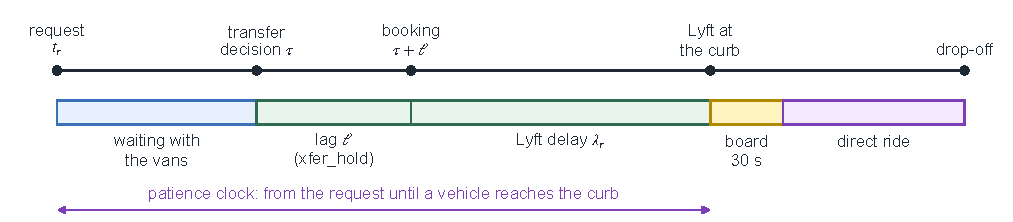
\includegraphics{figures/d_transfer.pdf}
\caption{Timeline of a transferred rider (not to scale). $t_r$ is the request time, $\tau$ the transfer decision, $\ell$ the ordering lag and $\lambda_r$ the rider's hidden Lyft delay; ``booking'' at $\tau+\ell$ is the Lyft order. The request leaves van planning at the decision; the Lyft is ordered one lag later and arrives after the rider's hidden delay. The patience clock keeps running from the original request until a vehicle reaches the curb; a transfer never resets it.}\label{fig:transfer}
\end{figure*}

% =====================================================================
\section{Experimental Design and Verification}\label{sec:design}

\textbf{Paired replay.} Each constructed night is replayed six ways, once per rule, with the same requests, places, parties, hidden patience and presence, Lyft delay per rider, and vans. Differences therefore reflect the rule within this specified model. Thirty nights replayed six ways are thirty \emph{paired} scenarios, not 180 independent nights. Pairing removes night-to-night differences from each comparison; it does not make the nights representative of April. Provisional pilot settings: 2-minute ordering lag; every Lyft offer accepted; 8.9\% no-show per arrival; placeholder patience; van travel $\times$ 1.2.

\textbf{Verification before interpretation.} Verification asks whether the code implements the specified model; validation asks whether the model represents the real service. We did the first, not the second (\cref{tab:verify}). We built small designed evenings with hand-computed answers and checked the simulator against them before scaling up; on three of them the simulator reproduces the hand-computed event times to the second. On one designed evening a separate brute-force program enumerated 292,181 plan combinations over the same candidates and always made the same choice as the MILP. The test suite has 253 passing tests, 168 of them written by separate AI review agents that did not reuse the simulator's code. AI wrote the simulator code and the checks under our direction; separate implementations are useful checks, but they share our assumptions and do not replace our own understanding of the model.

\begin{table}[t]
\centering\small
\caption{Verification evidence and numerical diagnostics for the pilot batch (180 runs).}\label{tab:verify}
\begin{tabularx}{\columnwidth}{@{}L@{}}
\toprule
Every run passed every per-run check; one code version for all runs\\
13,663 decision moments; the main solve was proven optimal over its candidates in all of them\\
41 moments had an incomplete search for equally good plans (a solver error); in all 41, full enumeration shows a unique optimum, the plan chosen\\
36 ride-time excess events (16 distinct requests on 10 nights); each coincided with a no-show wait on that van while the rider was aboard (an attribution check, not proof); 0 unexplained\\
Run time per run: mean 32 s, longest 253 s (Python, one core)\\
Reproducibility: 6 of 6 sampled reruns byte-identical\\
\midrule
\emph{Not validation:} do riders behave like our hidden draws? Do our evenings resemble real Homewood nights? Would the rules behave the same in operation?\\
\bottomrule
\end{tabularx}
\end{table}

% =====================================================================
\section{Preliminary Results}\label{sec:results}

All results in this section are \SIM{} outcomes on 30 constructed two-van burst nights under provisional rider behaviour. They describe the rules within this specified pilot; they do not rank them for real operations.

\subsection{Service: the predictive rules reached more requests}\label{sec:reach}
Our service measure is the share of \emph{all} 28 requests reached by a vehicle (van or Lyft curb arrival, not boarding) within 15 minutes. Riders who cancelled count as not reached, so the measure is not biased toward survivors. The two predictive rules reached about three quarters of requests within 15 minutes (0.73 and 0.75), against about half under vans only (0.48) (\cref{fig:reach}). The waiting-time rules barely moved it (0.50--0.51), and ``Unassigned for ten minutes'' did not (0.48). The predictive rules also ordered the most Lyft rides, about 9 to 10.5 per night. Measures without a threshold give the same ordering: requests picked up rose from 16.1 of 28 (vans only) to 20.2--20.4, and the 90th-percentile wait among those picked up fell from 20.2 to 12.2--13.3 minutes (\cref{tab:metrics}).

\begin{figure}[t]
\centering
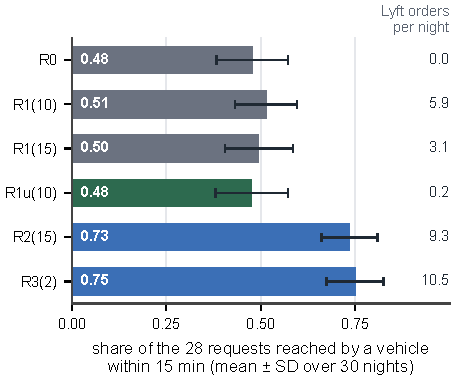
\includegraphics{figures/r3_reach.pdf}
\caption{Share of requests reached by a vehicle within 15 minutes, by rule (mean $\pm$ standard deviation (SD) across 30 nights), with Lyft orders per night at right. Blue: predictive rules; green: ``Unassigned for ten minutes''; grey: waiting-time rules. Codes as in \cref{tab:rules} \SIM.}\label{fig:reach}
\end{figure}

Two caveats keep this honest. First, the 15-minute measure favours early transfer. A request moved under ``Wait ten minutes'' has already waited at least 10 minutes, then faces the 2-minute lag and a Lyft delay with median 8 minutes, so it almost never reaches the curb within 15 minutes; under ``Wait fifteen minutes'', never. Second, the predictive rules used more Lyft, so this comparison does not isolate the benefit of \emph{prediction} at an equal Lyft budget. In practice the predictive rules transferred at the first decision moment at which the plan already predicted a long wait (median time waited at transfer: 0 s, against 629 s and 932 s for the two waiting-time rules). With a 2-minute lag and an assumed median Lyft delay of 8 minutes, a request moved at once usually reaches the curb within 15 minutes. So the gain on this measure largely reflects \emph{transferring early}, under our Lyft-delay assumption. Showing that the \emph{prediction} adds value needs a baseline that moves the same number of requests without reading the plan; that comparison is planned (\cref{sec:plan}).

\begin{table*}[t]
\centering\small
\caption{All measures by rule: mean of the 30 nightly values (standard deviation across nights) \SIM. Waits cover only requests picked up. The five outcome rows from ``Van trips completed'' to ``No-shows'' sum to the 28 requests. Transfers exceed Lyft orders by the requests cancelled during the 2-minute ordering lag. Thirty nights replayed six ways, not 180 independent nights.}\label{tab:metrics}
\begin{tabularx}{\textwidth}{@{}Lcccccc@{}}
\toprule
\textbf{Per night} & \textbf{R0} & \textbf{R1(10)} & \textbf{R1(15)} & \textbf{R1u(10)} & \textbf{R2(15)} & \textbf{R3(2)}\\
\midrule
Reached within 15 min (share of 28) & 0.48 (0.09) & 0.51 (0.08) & 0.50 (0.09) & 0.48 (0.10) & 0.73 (0.07) & 0.75 (0.08)\\
Requests picked up (of 28) & 16.1 (2.4) & 17.2 (2.6) & 16.5 (2.6) & 16.2 (2.5) & 20.2 (2.0) & 20.4 (2.3)\\
Wait median, min (per request picked up) & 8.6 (1.8) & 8.3 (1.6) & 8.4 (1.5) & 8.9 (2.1) & 7.5 (1.0) & 7.3 (1.0)\\
Wait 90th percentile, min (per request picked up) & 20.2 (5.3) & 18.1 (2.4) & 19.6 (4.0) & 20.2 (4.6) & 13.3 (1.5) & 12.2 (1.7)\\
Wait 90th percentile, min (per passenger picked up) & 20.1 (5.8) & 17.4 (2.7) & 19.2 (4.8) & 19.6 (4.7) & 13.2 (2.3) & 12.7 (2.7)\\
Van trips completed & 16.1 (2.4) & 14.1 (2.3) & 14.6 (2.4) & 16.1 (2.5) & 14.0 (2.7) & 13.3 (2.6)\\
Lyft trips completed & 0.0 (0.0) & 3.1 (1.4) & 1.8 (1.2) & 0.1 (0.3) & 6.2 (1.9) & 7.0 (1.6)\\
Cancelled waiting for a van & 10.8 (2.3) & 6.5 (2.3) & 8.9 (2.5) & 10.5 (2.4) & 3.3 (1.7) & 2.6 (1.5)\\
Cancelled after transfer & 0.0 (0.0) & 3.2 (1.8) & 1.5 (1.0) & 0.1 (0.4) & 3.1 (1.5) & 3.5 (1.5)\\
No-shows, van and Lyft & 1.1 (1.1) & 1.1 (1.0) & 1.2 (1.1) & 1.1 (1.1) & 1.4 (1.2) & 1.6 (1.3)\\
\midrule
Transfers decided & 0.0 (0.0) & 6.5 (1.6) & 3.5 (1.5) & 0.3 (0.6) & 9.8 (2.5) & 11.0 (2.0)\\
Lyft orders & 0.0 (0.0) & 5.9 (1.6) & 3.1 (1.4) & 0.2 (0.5) & 9.3 (2.5) & 10.5 (1.9)\\
Van-km (km driven by vans) & 51.2 (4.4) & 47.6 (5.5) & 48.6 (5.0) & 51.9 (4.8) & 45.7 (5.7) & 43.0 (4.0)\\
\bottomrule
\end{tabularx}
\end{table*}

\subsection{Moving a request to Lyft does not end its wait}\label{sec:fates}
A transferred rider still waits through the ordering lag and the Lyft's travel, and their original patience clock keeps running. \Cref{fig:fates} shows what happened to every transferred request. Under ``Wait ten minutes'', 95 of 196 transferred requests were cancelled before the Lyft arrived (18 during the ordering lag, 77 after the Lyft was ordered); under the predictive rules, about a third were. Riders moved by the predictive rules had usually waited less when transferred. Under our placeholder patience, where giving up becomes likelier with time waited, that is consistent with their lower share lost after transfer: a possible contributing mechanism, not an isolated cause, since the rules also differ in which riders they move. Whether the gap between policies survives other patience shapes is untested.

\begin{figure*}[t]
\centering
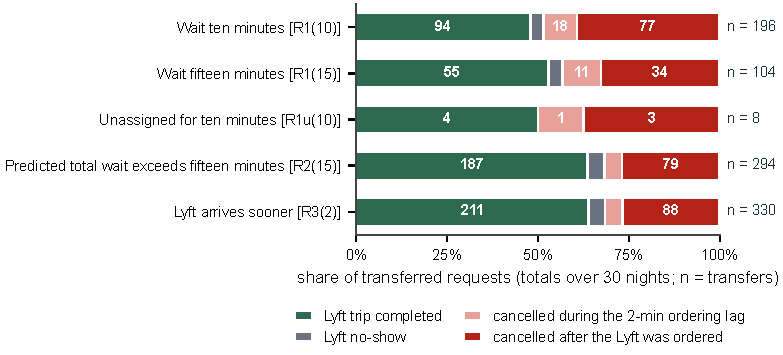
\includegraphics{figures/r4_fates.pdf}
\caption{What happened to transferred requests: totals over 30 nights, as shares of each rule's transfers (n). Each row reconciles: transfers = Lyft completed + Lyft no-show + cancelled in the lag + cancelled after the Lyft was ordered \SIM. ``Vans only'' makes no transfers and is omitted.}\label{fig:fates}
\end{figure*}

\subsection{Service and Lyft use point to different choices}\label{sec:tradeoff}
We keep two objectives separate: service (share reached within 15 minutes, higher is better) and Lyft use (orders per night, lower is better). A tested rule is \emph{dominated} if another tested rule is at least as good on both and strictly better on one. On the 30-night means, five of the six rules are nondominated (\cref{fig:tradeoff}). ``Vans only'' stays nondominated through zero Lyft use alone. ``Unassigned for ten minutes'' is dominated by ``Vans only'', but narrowly: its service is within about one request in 840 and it uses slightly more Lyft (it transferred 8 times in all, on 6 of the 30 nights). No noise margin (a minimum difference below which two rules count as tied) is applied yet, so in practice that is a near tie. Night by night, the two predictive rules reached more requests than vans only on all 30 nights; ``Wait ten minutes'' reached more on 19 and fewer on 6 (\cref{tab:nights}, appendix).

\begin{figure}[t]
\centering
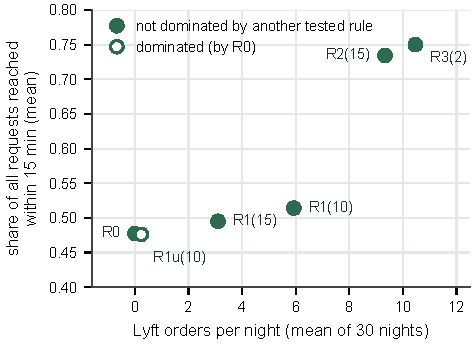
\includegraphics{figures/r7_tradeoff.pdf}
\caption{Lyft use against service, 30-night means for the six tested rules \SIM. Filled points are not dominated by another tested rule. Six tested points are not a frontier of all possible policies, and nondominated does not mean recommended.}\label{fig:tradeoff}
\end{figure}

\textbf{Reading the trade-off.} Nondominated does not mean recommended. Choosing among the nondominated rules requires a value judgement we have not made: how much extra Lyft use is one more rider reached worth? We also keep three trade-offs apart: the fixed weights inside the van objective (\cref{sec:milp}), the empirical trade-off between transfer rules (this section), and the decision criteria for choosing a rule, which the team has not yet agreed. For the same reason we have not yet attached confidence intervals: the primary metric, the margins and the paired comparisons are to be fixed together before any interval is computed, so they cannot be chosen after seeing the intervals.

% =====================================================================
\section{Approaches That Did Not Work, and What We Learned}\label{sec:failed}

\textbf{Replaying real nights.} The proposal's main evaluation depended on trip-level records. They did not arrive. \emph{Lesson:} aggregates do not identify individual journeys, but they constrain plausible evenings; labelling every number by how we know it lets us use them without overclaiming.

\textbf{The node-arc MILP as the runtime model.} The proposal formulated a node-arc model with routing, timing and Lyft variables. We did not adopt it as the runtime dispatcher. A convex piecewise-linear waiting penalty is not the obstacle (it is linear-programming representable with one epigraph variable per request); the obstacle is size, from timing variables and large-constant (``big-$M$'') precedence and time constraints, unrelated to our postponement constant $M$, that grow with vans and requests and must be re-solved every 2 minutes. Its Lyft term also created exactly the priority problem the feedback warned about. \emph{Lesson:} the route-selection MILP keeps the optimization exact over an explicit candidate set, keeps any waiting penalty linear, and makes the approximation (the candidate cap) visible and stated. The node-arc form survives only as a possible offline hindsight benchmark on tiny nights.

\textbf{A larger candidate set.} Allowing four new pickups per route made exact stop ordering take minutes per decision moment in Python. \emph{Lesson:} the cap $K=3$ is part of the held-fixed dispatcher and is reported with every result.

\textbf{The first postponement price.} It could make leaving a long-waiting party cheaper than serving them (\cref{sec:pending}). \emph{Lesson:} prices on ``not now'' decisions need the same physical realism as prices on served requests; we caught it only by tracing one decision by hand.

\textbf{Reading the dashboards.} Four proposal numbers were misread (\cref{tab:corrected}), and a no-show share was nearly applied with the wrong denominator (\cref{sec:noshow}). \emph{Lesson:} every derived number now carries its formula and its denominator.

\textbf{An earlier scenario ladder.} Our first batch of synthetic scenarios was generated before the team agreed what a scenario should contain. We paused it, studied how TransLoc and Hopkins dispatch actually operate, agreed a specification, and regenerated. \emph{Lesson:} agree the definition before generating data.

% =====================================================================
\section{Limitations and Assumptions}\label{sec:limits}

The findings are conditional on the evenings and behaviours we constructed. \Cref{tab:assumptions} ranks the assumptions by how much we expect them to matter.

\begin{table}[t]
\centering\small
\caption{Assumptions that could change the answer, in priority order.}\label{tab:assumptions}
\begin{tabularx}{\columnwidth}{@{}P{1.45cm}P{1.75cm}L@{}}
\toprule
\textbf{Assumption} & \textbf{Status} & \textbf{How it could change the interpretation}\\
\midrule
Rider patience & \ASM & A placeholder, and the one we expect to matter most (untested): it sets how many riders give up and the losses after transfer\\
Lyft delay & \ASM & A slower or more variable Lyft could weaken transfers; under placeholder patience, late transfers most\\
Workload and burst & \DER{} + \ASM & The pilot is deliberately heavy; at lighter load the rules may barely differ\\
Geography and matching & \ASM & Longer or more scattered trips change van reach and predicted pickups\\
Candidate restriction & \DES & At most 3 new pickups per van per decision; a richer search could change van performance and the rules' predictions\\
Fleet size & \DES & Two vans, not five; results may not scale\\
Dispatcher & \DES & Modelled on a 2016 vendor description, not verified Hopkins practice\\
\bottomrule
\end{tabularx}
\end{table}

Also open: the 15-minute measure favours early transfer; the pilot loses more requests to riders giving up (38.6\% under vans only) than April implies (23.7--35.6\%); the 8.9\% no-show rate depends on the status mapping and is reused for Lyft arrivals; Lyft is always available, every offer is accepted, and its delay does not depend on load or hour; Lyft cost is not modelled; demand is the burst pattern only, on one set of 30 nights; the per-rule results have no confidence intervals yet; and everything here is verification, not validation. Shorter outdoor waits are a service-quality proxy for the program's safety purpose; we do not measure safety.

% =====================================================================
\section{Plan for the Final Project}\label{sec:plan}

The next steps are ordered so that we test robustness before fine-tuning a winner (\cref{fig:roadmap}). A threshold tuned to placeholder behaviour could be tuned to our assumptions rather than to the service.

\begin{figure*}[t]
\centering
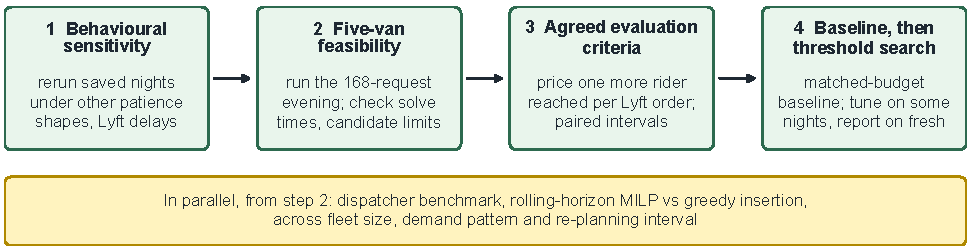
\includegraphics{figures/r6_roadmap.pdf}
\caption{Plan for the final, in order (all planned, not yet run). Step 4 combines the matched-budget baseline and the threshold search (items 4 and 5 below). The dispatcher benchmark runs alongside, from the five-van step.}\label{fig:roadmap}
\end{figure*}

\begin{enumerate}\setlength\itemsep{2pt}
\item \textbf{Behavioural sensitivity.} Rerun the saved nights under other patience shapes (Weibull shape 1 and 2, other medians) and Lyft delays (median 5 / 8 / 12 minutes). Does the gap between rules survive, and which patience shapes bring the vans-only give-up share inside April's range?
\item \textbf{Five-van feasibility.} Build and run the 168-request, five-van evening; check solve times and whether the candidate cap binds.
\item \textbf{Agreed evaluation criteria.} Decide how much extra Lyft use one more rider reached is worth, and fix non-inferiority margins (the largest loss in service we would accept in exchange for less Lyft use); then compute paired confidence intervals across nights. Report service at 10 and 20 minutes as well as 15.
\item \textbf{Matched-budget baseline.} Add a rule that moves the same number of requests per night without reading the plan (for example, a random set of requests on arrival). Only the gap between the predictive rules and this baseline measures the value of prediction.
\item \textbf{Threshold search.} Only then, search a finite set of thresholds for each rule family, tuning on one set of nights and reporting on fresh seeds, so the reported result is not fitted to the nights it was tuned on. This finds the best option within a finite set, not over all policies.
\item \textbf{Dispatcher benchmark (answering the feedback).} On identical nights, compare the rolling-horizon MILP with a greedy insertion dispatcher (the trade-off studied at scale in [6]) (insert each new request at its cheapest position on arrival; never reassign), across fleet size (4 to 7 vans on the same requests), demand pattern (base, burst, far-trip, high load) and re-planning interval (60 / 120 / 300 s), with the transfer rule held fixed (vans only first, then the adopted rule). Design: 30 paired nights per cell, the same service measure and Lyft count as above, and paired differences with intervals. The two-van runs took 32 s on average (longest 253 s) in Python, so five-van run times are measured first, in step 2. We also re-check the adopted postponement price on these nights. This measures under which demand and fleet conditions coordinated re-optimization pays off, and whether the dial-a-ride structure makes it valuable here.
\end{enumerate}

\textbf{A possible extension.} Choosing the transfer policy could itself be posed as a leader--follower (bilevel) problem [7]: a policy designer chooses the rule and threshold, and the routing dispatcher responds. It is bilevel because the dispatcher's response to each transfer changes the outcomes the designer is judged on. To state it precisely we would still need to define the leader's choices, whether the follower is one decision moment or a whole evening, how ties in the follower's response are treated, the expectation over constructed nights, the loss and its weight on Lyft use, and any budget or service-floor constraints. A finite search over our sampled nights would find the best option in a finite set for those nights, not for the true expectation or all policies. It is proposed, not implemented.

\textbf{Timeline.} \emph{Early November:} behavioural sensitivity on the saved nights; agree evaluation criteria with the professor. \emph{Mid November:} five-van evening and dispatcher benchmark. \emph{Late November:} matched-budget baseline and paired intervals, then the threshold search. \emph{December:} final report, presentation and a short summary for JHU Transportation.

% =====================================================================
\section{Conclusion}\label{sec:conclusion}

Two statements are defensible today. First, aggregate data did not give us individual journeys; it gave us constraints for building plausible evenings, and every input now says how we know it. Second, within our specified pilot, transfer rules that moved requests to Lyft as soon as the van plan predicted a long wait improved timely curb arrival while using more Lyft; whether the prediction itself adds value at an equal Lyft budget is still to be tested. Choosing a policy requires testing the assumptions and deciding what trade-off is acceptable. These results were tested in simulation, on 30 constructed two-van nights; they are not a policy recommendation.

% =====================================================================
\section*{References}

{\small
\begin{enumerate}\itemsep 2pt \parskip 0pt
\item Cordeau, J.-F. (2006). A Branch-and-Cut Algorithm for the Dial-a-Ride Problem. \emph{Operations Research}, 54(3), 573--586.
\item Cordeau, J.-F., \& Laporte, G. (2007). The Dial-a-Ride Problem: Models and Algorithms. \emph{Annals of Operations Research}, 153, 29--46.
\item Ho, S. C., Szeto, W. Y., Kuo, Y.-H., Leung, J. M. Y., Petering, M., \& Tou, T. W. H. (2018). A Survey of Dial-a-Ride Problems: Literature Review and Recent Developments. \emph{Transportation Research Part B: Methodological}, 111, 395--421.
\item Alonso-Mora, J., Samaranayake, S., Wallar, A., Frazzoli, E., \& Rus, D. (2017). On-Demand High-Capacity Ride-Sharing via Dynamic Trip-Vehicle Assignment. \emph{Proceedings of the National Academy of Sciences}, 114(3), 462--467.
\item Berbeglia, G., Cordeau, J.-F., \& Laporte, G. (2010). Dynamic Pickup and Delivery Problems. \emph{European Journal of Operational Research}, 202(1), 8--15.
\item Bertsimas, D., Jaillet, P., \& Martin, S. (2019). Online Vehicle Routing: The Edge of Optimization in Large-Scale Applications. \emph{Operations Research}, 67(1), 143--162.
\item Colson, B., Marcotte, P., \& Savard, G. (2007). An Overview of Bilevel Optimization. \emph{Annals of Operations Research}, 153(1), 235--256.
\item Huangfu, Q., \& Hall, J. A. J. (2018). Parallelizing the Dual Revised Simplex Method. \emph{Mathematical Programming Computation}, 10(1), 119--142. (HiGHS solver.)
\item Luxen, D., \& Vetter, C. (2011). Real-Time Routing with OpenStreetMap Data. \emph{Proceedings of the 19th ACM SIGSPATIAL International Conference on Advances in Geographic Information Systems}, 513--516. (OSRM.)
\item TransLoc TechLog (2016). Ridesharing Algorithms in TransLoc OnDemand. Archived copy, April 2018. Historical description of the vendor's engine.
\item Johns Hopkins University Facilities \& Real Estate. Shuttle Services and Night Ride pages. \url{https://jhfre.jhu.edu/ts/transportation/}\linebreak[0]\url{shuttle-services/} (archived captures 2023--2026; live page read 21 October 2026).
\item JHU Transportation (2026). Blue Jay Night Ride operations dashboards, April 2026 (TransLoc). Restricted; used in aggregate only.
\item Deming, W. E., \& Stephan, F. F. (1940). On a Least Squares Adjustment of a Sampled Frequency Table When the Expected Marginal Totals Are Known. \emph{Annals of Mathematical Statistics}, 11(4), 427--444. (Iterative proportional fitting.)
\end{enumerate}
}

\section*{AI-Use Disclosure}

\textbf{Team members.} Irfan Setiadi, Miles Zhou, Youzhi Zhang, Vignesh Rajesh Babu.

\textbf{Tools used.} Anthropic Claude (Claude Code) and OpenAI Codex.

\textbf{Purpose.} We used these tools to help digitize the April dashboards, draft and review the scenario specification and decision log, write the scenario generator, the simulator and the dispatcher code under our direction, write independent verification tests through separate review agents, produce the figures, and organize and draft this report and the midterm slides.

\textbf{How the output was used.} AI-generated code, figures and text were reviewed and revised by the team before use. Design decisions (scope, objective, rules, assumptions) were made by the team and are recorded in our decision log; AI tools proposed options and drafted text.

\textbf{Verification.} Simulator behaviour was checked against hand-computed answers on small designed evenings, a separate brute-force enumeration, and 253 automated tests; every number in this report was cross-checked against the saved simulation outputs and the April aggregates. We remain responsible for the accuracy, originality and integrity of the submitted work, and every team member is expected to be able to explain it.

% =====================================================================
\appendix
\onecolumn
\section{Night-by-Night Trade-off}\label{app:nights}

\begin{table}[h]
\centering\small
\caption{Trade-off night by night \SIM. A rule that makes no transfer on a night replays vans only exactly; identical results do not dominate each other, so both count as not dominated. Above / below counts are paired comparisons on the same constructed night, with no intervals yet.}\label{tab:nights}
\begin{tabular}{@{}llccccc@{}}
\toprule
\textbf{Rule} & \textbf{Code} & \textbf{\shortstack{Reached\\(mean)}} & \textbf{\shortstack{Lyft orders\\(mean)}} & \textbf{\shortstack{Nights not\\dominated}} & \textbf{\shortstack{Nights identical\\to vans only}} & \textbf{\shortstack{Nights above / below\\vans only}}\\
\midrule
Vans only & R0 & 0.477 & 0.00 & 30 of 30 & 30 & 0 / 0\\
Wait ten minutes & R1(10) & 0.514 & 5.93 & 11 of 30 & 0 & 19 / 6\\
Wait fifteen minutes & R1(15) & 0.495 & 3.10 & 14 of 30 & 1 & 15 / 5\\
Unassigned for ten minutes & R1u(10) & 0.476 & 0.23 & 26 of 30 & 24 & 2 / 2\\
Predicted total wait $>$ 15 min & R2(15) & 0.735 & 9.33 & 24 of 30 & 0 & 30 / 0\\
Lyft arrives sooner & R3(2) & 0.750 & 10.47 & 12 of 30 & 0 & 30 / 0\\
\bottomrule
\end{tabular}
\end{table}

\section{The MILP Constant and Solver Settings}\label{app:milp}
At each decision moment, with $b_r^{\max}$ an upper bound on $b_r$ computed at that moment ($0 \le b_r \le b_r^{\max}$), the postponement constant is
\[
M = 1 + \sum_v \Bigl(\max_k c_{vk} - \min_k c_{vk}\Bigr) + \sum_r b_r^{\max},
\]
so a plan that postpones $j$ fewer requests gains at least $jM$, more than any possible difference in route costs and postponement terms. Route costs are scaled to integers, so the ``$1+$'' term and an absolute gap below one cost unit preserve this ordering. Every proven-optimal plan therefore postpones the fewest requests the candidate set allows (checked by full enumeration on a designed evening). Solver: HiGHS, one thread, fixed seed, relative gap 0, absolute gap below one cost unit, node limit 100,000, and $\Psi = 1000$ points per passenger-minute over the guardrail. If the node limit is reached, the best plan found is executed and labelled feasible but unproven; this never occurred in the pilot.

\section{Event Order Within One Second}\label{app:order}
The simulator clock counts whole seconds from 18:00. Events in the same second are applied in this order: drop-offs; curb arrivals (stopping the patience clock); service ends; vans on or off duty; new requests; patience checks; Lyft orders; the decision moment; departures. A van commits to a stop when it departs toward it, and a committed request is not eligible for transfer. After a transfer come a 2-minute ordering lag and then the rider's hidden Lyft delay; the rider may cancel at any point before the Lyft reaches the curb. Presence is one draw per rider, used whichever vehicle arrives.

\end{document}
